% !TeX root = ../main.tex

\chapter{Datasets} \label{chapter:datasets}

This chapter presents all datasets that are going to be used in the following evaluation. Three different video datasets have been chosen that were used in related works in order to be able to compare the results and analyze the strength and weaknesses of different network models. The selected datasets will be introduced one after another ordered by the content complexity with respect to the possible variations in color, motion and physical environment. Additionally, random samples from each dataset will be shown to get a better idea of how the data looks like that is fed to the network.


\section{Moving MNIST} \label{sec:ds_mm}


We first train our model on a synthetic dataset of black and white images with flying handwritten digits. The \textit{Moving MNIST} has been introduced in \parencite{unsup_learn_lstm} and applied in context of video frame prediction. Since then, it has been used several times in different follow-up works like \parencite{spat_temp_video_autoenc} or \parencite{conv_lstm_nowcasting}. 

\subsection{Characteristics and Data Generation}

In the proposed setting, each sequence consists of $20$ image frames of size $ 64 \times 64 $ with two random moving digits from the MNIST\footnote{MNIST dataset of handwritten digits: \url{http://yann.lecun.com/exdb/mnist/}} dataset in it. One major advantage of this simple dataset is that it exhibits a nearly unlimited size, because it can be generated on the fly. When training a model, we therefore randomly choose two random digits from the first \num{55000} digits of the training set and place them on any location of the first image patch. For the generation of subsequent frames, a velocity is assigned to each digit, whose direction is chosen uniformly from a unit circle. Further, the simple physical rule is applied that the angle of incidence is equal to the angle of reflection when any digit of size $ 28 \times 28 $ touches the wall. Moreover, this enables other interesting properties of the dataset, such as basic dynamics due to having to predict the right trajectory after bouncing off a wall, as well as multiple occlusion effects of overlapping digits. Consequently, even that the generation process of the dataset is that simple, it is hard for a model to generate accurate predictions on the test set without learning a representation that encodes the internal motion of the system \parencite[p. 6]{conv_lstm_nowcasting}. Last but not least, having a simpler dataset at hand allows us to gain a better understanding of the model's behavior in respect to its hyperparameters. Especially in consideration of the very long training time of several days when more complex or even natural videos are used.

\begin{figure}[htpb]
\centering
\begin{subfigure}{1.0\textwidth}
  \centering
  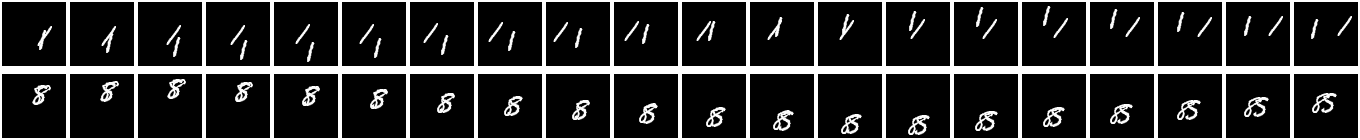
\includegraphics[width=1.0\linewidth]{figures/ds/mm_train.png}
  \caption{Training set}
  \label{fig:mm_train}
  \vspace{.1cm}
\end{subfigure}
\begin{subfigure}{1.0\textwidth}
  \centering
  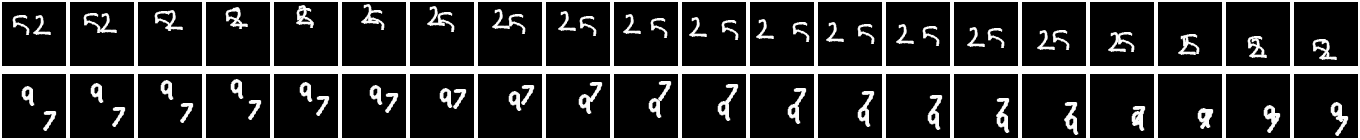
\includegraphics[width=1.0\linewidth]{figures/ds/mm_valid.png}
  \caption{Validation set}
  \label{fig:mm_valid}
  \vspace{.1cm}
\end{subfigure}
\begin{subfigure}{1.0\textwidth}
  \centering
  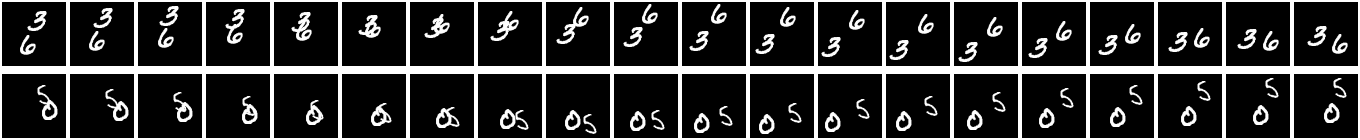
\includegraphics[width=1.0\linewidth]{figures/ds/mm_test.png}
  \caption{Test set}
  \label{fig:mm_test}
\end{subfigure}
\caption[MovingMNIST Image Sequence Samples]{Randomly chosen samples of generated image sequences of size $64 \times 64$ from the Moving MNIST dataset.}
\label{fig:moving_mnist}
\end{figure}

The generation procedure of the validation set is equal to the previously described process to create the training data, but with the difference that the last \num{5000} digits of the original MNIST training split is used. On the contrary, the test set is not generated by using the MNIST test split. Instead, the pre-generated test set of \parencite{spat_temp_video_autoenc}\footnote{Pre-generated MovingMNIST test set with \num{10000} sequences: \url{http://mi.eng.cam.ac.uk/~vp344/}} that contains exactly \num{20} frames long sequences with \num{10000} examples has been used. In this way, more comparable results can be achieved to at least one competing model. A random sample from each of these splits is presented in Figure \ref{fig:moving_mnist}.

Even that some other works have used a fixed number of pre-generated frame sequences only, we kept up with the on-the-fly generation process of the initial paper for at least three reasons. First, it limits the amount of data and therefore increases the chance of overfitting. Seconds, loading the pre-generated frames from disk takes more time than generating them on the fly; hence it could have a slightly negative impact on the overall training time. And third, it reduces the total memory requirements in case the whole data would otherwise be pre-loaded into memory in order to eliminate the second mentioned issue.

\subsection{Data Preprocessing}

Since the original pixel values of the MNIST dataset are in a range of $[0, 255]$, we perform simple rescaling to $[0, 1]$ in order to normalize the data. Further, subtracting the mean pixel-values has been considered as well because gray-scale images have the stationarity property\footnote{For example when the statistics for each data dimension follows the same distribution, the data is said to be stationary.}. But due to the fact that this is not often done in practice when the MNIST dataset is used \parencite{stanford_data_pre}, as well as we could not see any noticeable improvements when applying it, caused that mean subtraction is not applied while preprocessing the data. Moreover, one can belief that since most parts of any image is black (and therefore zero), further processing of the data is not necessarily required.

Additionally, instead of feeding the model with continuous floating values in the normalized range, binary pixel values are used only. This decision results from the use of binary cross-entropy as the main loss function for this dataset, which has shown to be the favorable choice for image generating models with MNIST \parencite{unsup_learn_lstm}, \parencite{conv_lstm_nowcasting}. Therefore, every pixel $p$ is set to zero if $p < \num{0.5} $, and a value of one is assigned to all other pixels. Moreover, the sigmoid activation function is used in the output layer in order to support the saturation of all pixels into either zero or one.

\section{MsPacman} \label{sec:ds_pac}

In order to accommodate the request of assessing our model on more complex data compared to the previously presented dataset, but which still has negligible dynamics compared to natural clips, a second data collection is used that consists of video game recordings. The \textit{MsPacman}\footnote{MsPacman dataset: Generated by \href{mailto:jun_ki_lee@brown.edu}{\textit{Jun Ki Lee}} in a student project at Brown University by taking recording the classical video game.} dataset has been used in an independent TensorFlow implementation of \parencite{deep_multiscale_video_pred}\footnote{Adversarial video generation in TensorFlow:\\ \url{https://github.com/dyelax/Adversarial_Video_Generation}} for adversarial video generation and future frame prediction. It contains several interesting dynamics and properties that make it a reasonable choice to be considered in the evaluation of our model. These will be discussed in more detail in the course of this section.

\subsection{Characteristics}

This video game dataset contains about half a million single images of size $ 160 \times 210 $. These images can be grouped into \num{517} game recordings for the trainging set and $51$ recordings for the test set. Each recording has a variable length and ranges from about \num{500}-\num{1500} frames per sequence. The last \num{51} sequences of the training data are taken for the validation set to have it roughly the same size as the testing set. Thus, it ends up with a total number of \num{418287} frames for training, \num{45007} images for validation and \num{46380} images for testing.

The action inside each recording acts in a closed world with various game rules that the network has to understand. Just to name some example, all objects follow the path between the walls of the game world, with the two exceptions that ghosts in the center might exit the cave through the top barrier, as well as that Pacman can teleport himself by leaving the world using its left or right exit. Further, the game's main character opens and closes its mouth, can eat the distributed dots, fruits or blue ghosts. Some recordings from the different dataset splits are depicted in Figure \ref{fig:pacman_full}.

\begin{figure}[htb]
\centering
\begin{subfigure}{1.0\textwidth}
  \centering
  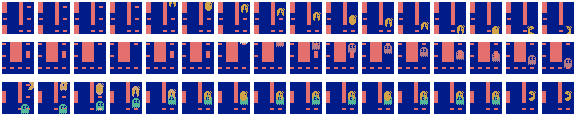
\includegraphics[width=1.0\linewidth]{figures/ds/pac_train.png}
  \caption{Training set}
  \label{fig:pac_train}
  \vspace{.1cm}
\end{subfigure}
\begin{subfigure}{1.0\textwidth}
  \centering
  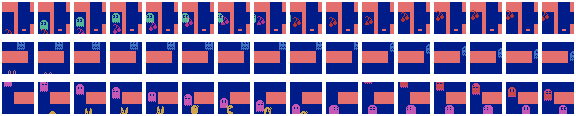
\includegraphics[width=1.0\linewidth]{figures/ds/pac_valid.png}
  \caption{Validation set}
  \label{fig:pac_valid}
  \vspace{.1cm}
\end{subfigure}
\begin{subfigure}{1.0\textwidth}
  \centering
  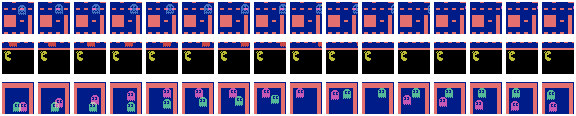
\includegraphics[width=1.0\linewidth]{figures/ds/pac_test.png}
  \caption{Test set}
  \label{fig:pac_test}
\end{subfigure}
\caption[MsPacman Crop Image Samples]{Example sequences from different splits of the used MsPacman dataset. These randomly selected frames have been cropped to $32 \times 32 $ and filtered to ensure enough movement while training the model.}
\label{fig:pacman}
\end{figure}


\subsection{Data Preprocessing} \label{sec:pacman_preprocessing}

The images of every sequence are rescaled to be in range of [-1, 1]. To ensure that the predicted outputs exhibit the same value scale, a $tanh$ activation function is used after the last transposed convolutional layer. Since each single image is quite big, we take advantage from our fully-convolutional approach and train the network on random crops of size $ 32 \times 32 $ only. Some random samples of these cropped images are shown in Figure \ref{fig:pacman}. Unfortunately, the usage of small image crops follows that most of the used training sequences show no motion at all.

After experiencing a strong preference of predicting the worlds background over the small moving objects only, we decided to use a technique similar to \parencite{deep_multiscale_video_pred} in order to ensure that each temporal sequence shows enough movement. Therefore, each time when a random part of the sequence is selected from the training set, the $\ell_2$ difference between each consecutive frame pair is calculated. Afterwards, this randomly chosen cropped sequence is rejected until the overall movement of the input sequence is higher than a given threshold of $25 \cdot n_{frames}$, or a specified repetition limit is reached in order to prevent an endless loop. Additionally, it is checked that there is also movement at the end of the input sequence to ensure that the whole movement is not just taking place at the beginning of the whole sequence only. Further, it reduces the chance that the network has to guess the movement of objects that enter the patch after the prediction-decoder has taken over, which it obviously cannot predict. Last but not least, the input and output sequence length has been slightly shortened compared to the other two datasets to \num{8} frames each. The reason for this is that this performed motion detection is kind of useless when being applied on too long sequences, because of the high chance that all these fast moving objects within the selected crop have already left the scene too quickly. However, even that this filtering of the final training examples sounds quite radical, it is to highlight that a high fraction of the input space is still static content. This can be attributed to the use of convolutional layer with small windows sizes that slide over the input space.

\subsection{Data Augmentation}

In terms of data augmentation, the brightness or contrast of the image examples is \textit{not} randomly modified, because it does not make sense in context of this video game which uses a fixed set of colors only. But since the game world is mirrored horizontally, random horizontal flipping is performed in case the chosen crop is not showing any parts of the status display at the bottom. Furthermore, we iterated over all sequences \num{256} times per epoch, reasoned by the fact that the dataset consists of only a few but very long sequences. A second reason is that a very short clip and a small random crop from these frame sequences is used only. 


\section{UCF-101} \label{sec:ds_ucf}

Finally, a third dataset is used to examine if the model can also deal with complex, natural videos. Therefore, the \textit{UCF-101} dataset \parencite{ucf}\footnote{UCF-101 dataset and further information: \url{http://crcv.ucf.edu/data/UCF101.php}} is used. With its \num{13320} clips and about \num{27} hours of video data, it belongs to the largest labeled dataset for human action recognition. The dataset is made of user-uploaded videos that can contain overloaded background or camera movement. All \num{101} categories can be divided into \num{25} main groups,  where each video from the same group shares similar features, such as an roughly equal viewpoint. The action categories can also be separated into five types, namely human-object interaction, body-motion only, human-human interaction, playing musical instruments and sports. Even that this dataset was originated for human action recognition, it can be used in context of frame prediction as well by simply using the raw video data only.

Before taking a deeper look into the characteristics and applied preprocessing steps, it is to add that there exists an even larger video dataset for the purpose of representation learning. This huge dataset is called \textit{Sports-1M} and contains over \num{1.1} million YouTube video links of \num{478} classes that have been annotated in an automated process \parencite{large_video_class}. But due to infrastructural issues with such a huge dataset, as well as a tremendous time exposure regarding data preprocessing, we decided to not use it in this thesis.


\subsection{Characteristics}

The average video length of the whole dataset is about \num{6.2} seconds, while each single can range from about \num{1} second to a maximum of \num{71} seconds. Even that the initial paper states that each video has a fixed resolution and frame rate of $ 320 \times 240 $ and \num{25} FPS respectively, we experienced that a handful of videos exhibit a slightly different resolution. Consequently, these frames have been padded with zeros or cropped in the center to end up in an equal size for all videos. Such a padded video, as well as other example clips, can be seen in Figure \ref{fig:ucf_valid_full}.

The dataset provides three standards train/test splits intended to be used for either action recognition or action detection. We have chosen the third standard split for action recognition, because it consists of the most videos for training, as well as allowed the simplest divisibility of the test split. Since we expect that a huge training set is fundamental for the network in order deeply explore the inner dynamics, we decide to take the validation data from the test split instead of the training data as usual. For the avoidance of doubt, other previous works using UCF-101 for frame prediction either have only used $ 10\% $ of the test set actually for testing \parencite[p. 12]{deep_multiscale_video_pred}, or did not make any comment about which data partitions they have chosen for validation and testing. Finally, it therefore ends up with \num{9624}, \num{1232} and \num{2464} videos for the training, validation and test set, respectively.


\subsection{Data Preprocessing}

The data preprocessing that is performed in UCF-101 is very similar to the procedure describe in Section \ref{sec:pacman_preprocessing}, but with the following differences. First, the width and height of all images are cut in half, resulting in downscaled videos of size $160 \times 120$ using linear interpolation. This is done in order to compensate the noisy, pixelated artefacts in the videos. Also, it increases the chance of finding a random crop of size $ 32 \times 32 $ that actually has some true motion in it, instead of just flickering caused by noise. Second, the constraint regarding motion filtering when selecting the crop region of the randomly selected clip has been slightly weaken. While a sequence that has a very low motion in the input frames is still rejected, it does not dismiss a sequence that has no motion at the end. Figure \ref{fig:ucf} shows several cropped sequence examples from the different dataset splits that are fed into our model.

\begin{figure}[htb]
\centering
\begin{subfigure}{1.0\textwidth}
  \centering
  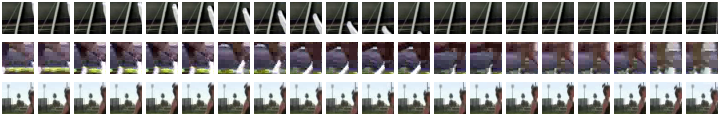
\includegraphics[width=1.0\linewidth]{figures/ds/ucf_train.png}
  \caption{Training set}
  \label{fig:ucf_train}
  \vspace{.1cm}
\end{subfigure}
\begin{subfigure}{1.0\textwidth}
  \centering
  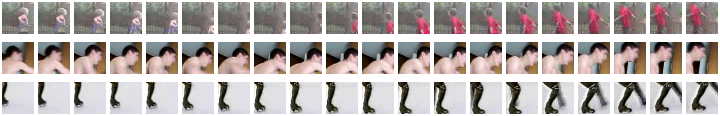
\includegraphics[width=1.0\linewidth]{figures/ds/ucf_valid.png}
  \caption{Validation set}
  \label{fig:ucf_valid}
  \vspace{.1cm}
\end{subfigure}
\begin{subfigure}{1.0\textwidth}
  \centering
  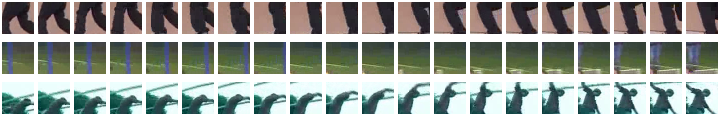
\includegraphics[width=1.0\linewidth]{figures/ds/ucf_test.png}
  \caption{Test set}
  \label{fig:ucf_test}
\end{subfigure}
\caption[UCF-101 Crop Image Samples]{Sequence examples from UCF-101. These frames have been randomly selected from the different splits, cropped to $32 \times 32 $ and filtered to ensure they contain at least a small proportion of motion.}
\label{fig:ucf}
\end{figure}

Furthermore, because it is wasteful to load the whole video file into memory, especially in regard that only a very small portion of the data is actually used to generate a single example for the next batch, an additional offline preprocessing of the data is performed before the actual training process starts. For that reason, it iterates over all raw video files and generates non-overlapping binary video sequences with a length of \num{30} frames each. Fortunately, the generated files can be reused after doing this process once. Finally, it ends up with \num{55150} clips for the training set, \num{7183} clips for the validation set and \num{14451} clips for the test set.


\subsection{Data Augmentation}

Regarding data augmentation, the contrast and brightness of the overall image sequence is randomly modified by a delta of $ \pm20\% $. Further, random horizontal flipping is performed for the training data. While the contrast or brightness in the validation or test data is not randomly changed, we double their size by using both the normal and the flipped instances. Further, four crops from every video are used in each evaluation iteration in order to have a balance between more consistent evaluations and still an acceptable processing time. It is to add that these augmentation steps are performed on-the-fly. To facilitate this, an advanced double-buffered input queue is used. The first \textit{filename queue} is randomly filled with references to the binary sequence files generated before. Afterward, \num{16} CPU threads dequeue a reference from this queue, load the sequence into memory and then perform all preprocessing steps in parallel, for the purpose of generating a single training example. Finally, this example is then pushed to the \textit{shuffled batch queue}, from which the model loads its batches in every iteration. Consequently, there is no waiting time in-between each training step.
